% !TEX root = ../thesis.tex
\chapter[Tycho's Six]{Tycho's Six: High Resolution~spectroscopy search for the remaining donor of the Tycho supernova}
\label{chap:sn1572_hires}
\emph{\small This Chapter is being prepared for publication as `Tycho's Six: High-Resolution spectroscopy search for the remaining donor of the Tycho supernova' - 
Kerzendorf, W. E., Schmidt, B. P., Yong, D., Jeffery,~C.S. ,  Anderson, J.P., Nomoto, K., Podsiadlowski,  Ph., Simon, J.D., Gal-Yam, A., Silverman, J.M., Filipenko, A.V., Murphy, S.J., Bessell, M.S.}

\section{Introduction}
\label{sec:sn1572_hires:introduction}

\glspl{snia} are of great interest for astronomy. They represent some of the most extreme physical situations in stellar astronomy, produce substantive amounts of \gls{ige} which impacts the chemical evolution of galaxies and the Universe, and are uniquely powerful cosmic distance probes. Despite their wide ranging significance, fundamental uncertainties remain around the progenitor of these cataclysmic events. 

There is general consensus that \sneia\ are caused by the deflagration/detonation of a \gls{cowd} which is accreting material from a binary companion. Scenarios exists where the explosion can be initiated from a detonation on the surface of the star \citep{1995ApJ...452...62L, 2010A&A...514A..53F}, through runaway carbon burning in the white dwarf's interior, or through a cataclysmic merger of objects.

Observationally, two main scenarios for this accretion process can be identified. The \gls{sds} sees the accretion process occurring through \gls{rlof} of a close non-degenerate companion (also known as \gls{donor} star). This companion, which has undergone common envelope evolution with the white dwarf, can be a helium, main-sequence, sub-giant, or red giant star. In all cases the donor star should survive the explosion and remains visible post-explosion. 

The second scenario is the  dynamical merger of two white dwarfs (\gls{dds}). In this scenario, the co-evolution of two stars eventually leads to a close binary of two white dwarfs, which are able, through the emission of gravitational radiation, to merge over a wide range of times after the initial formation of the system. In most cases this would leave no remaining star \citep[e.g.][]{2010Natur.463...61P}.

Both scenarios have support in observation and theory. The detection of circumstellar material around certain \gls{snia}, such as \sn{2006}{X}\ \citep{2007Sci...317..924P}, provides support for the \gls{sds}. On the other hand the lack of substantial hydrogen in in the majority of other \sneia\ \citep{2007ApJ...670.1275L} poses a challenge to the \gls{sds}.


\citet{2010ApJ...708.1025K} suggests that the interaction with the non-degenerate companion should imprint an observable signature on a SN Ia  light curve, depending on viewing angle, and radius of the companion. Such an excess has not yet been observed \citep{2010ApJ...722.1691H, 2011Ap&SS.tmp...40T, 2011arXiv1106.4008B} which is at odds with \gls{redgiant} companions forming the majority of \sneia.

Population synthesis calculations are challenging, with various authors getting different results for the same inputs (Nelemans paper, which??). However there is a general trend from these calculations that neither single-degenerate nor double degenerate stars can provide enough systems to explain the \gls{snia} rate \citep{2009ApJ...699.2026R, 2010A&A...515A..89M,2010A&A...521A..85Y,2008ApJ...677L.109H}. Several authors suggest the population might comprise both single and double degenerate systems.

The physics of white dwarf mergers is challenging to simulate numerically, but in the simplest calculations, these mergers will lead to the formation of a neutron star via an electron capture, rather than a thermonuclear explosion \citep{1985A&A...150L..21S}. Recently \citet{2010Natur.463...61P} have shown that for certain parameters (white dwarf binaries with a mass ratio very close to one) the merger may explain sub-luminous supernovae (e.g. \gls{91bg} \glspl{snia}), although \citet{2011arXiv1101.5132D} note that the initial conditions of the system may change these conclusions.

To investigate the nature of progenitors observationally \rl\ have tried to directly detect donor stars in \snia\ remnants within the Milky Way. They have identified two historical Galactic \glspl{sn} well suited to this task - \sn{1006}{}\ and \sn{1572}{} (Tycho's SN). Both remnants are young (440 and 1000~years old, respectively), almost certainly \gls{snia} from both their observational signatures \citep{2006ApJ...645.1373B,2004ApJ...612..357R} and not overwhelmed by Galactic extinction. In this paper, we will focus on \sn{1572}{}. 

\snr{1572} is relatively close ($2.8\pm0.8$\,\kpc), very young and has been confirmed as a normal \snia\ remnant both from the remnant \citep{2006ApJ...645.1373B} and from a light echo \citep{2008Natur.456..617K}. 


\rl\ investigated most bright stars in the central regions of \sn{1572}{}\ and found a star with an unusual spatial motion (\starg\ by their nomenclature) and suggested this as a possible donor star for \sn{1572}{}. While the star has an unusual spatial motion compared to other stars in the field, its current location and proper motion place it a significant distance from the remnant's center - a feature difficult to explain in connecting \starg\ to \snr{1572}{}. One consequence of \gls{rlof} is a rotational velocity induced on the \gls{donor} star by tidal locking in the system. This results in an unusually large rotationally velocity, related to the orbital velocity of the binary system and can be used to single out donor stars against nearby unrelated stars. \wek\ investigated rotation for  \starg\ but found no excess rotation velocity compared to a normal star. \wek's measurements of \starg, including a revised radial velocity, compared to a Galactic models, showed it is statistically consistent with an interloping star. However, \wek\ were able to provide an a priori unlikely scenario, where the star was able to lose its rotational signature. 

\gh\ analysed a spectrum of \starg\ observed with the \gls{hires} instrument on the Keck telescope. In addition to confirming \wek's radial velocity for \starg, \gh\ determined its stellar parameters and metallicity. \gh\ concluded that \starg\ has an unusually large amount of nickel. \gh\ claim that this enhancement in nickel can be attributed to the accretion of ejecta material on the \gls{donor} star during the explosion. 

In this paper we analyse \gls{hires} spectra of the six bright stars in \snr{1572}{} center. These spectra were taken by the same program that obtained the data used by \gh\ and we independently reanalyze this spectrum as part of our program. We describe the observational data and our data reduction procedures in Section \ref{sec:sn1572_hires:observ-data-reduct}. Section \ref{sec:analysis} is divided into five subsections detailing the measurements of proper motion, radial velocity, rotation, stellar parameters and abundances. In Section \ref{sec:sn1572_hires:discussion} we analyse the measurements of each star to investigate its potential association with \snr{1572}, and present our conclusion in section \ref{sec:sn1572_hires:conclusion}.

\section{Observations and Data Reduction}
\label{sec:sn1572_hires:observ-data-reduct}

We obtained spectra with the \gls{hires} on the Keck 10m telescope on Mauna Kea. The observations were made on two nights on 2006 September 10 and 2006 October 11.  The slits B5 and C1 (with the same width of 0.86\arcsec\ but different lengths, B5 length 3.5\arcsec, C1 length 7.0\arcsec) were used resulting in a wavelength coverage of 3930--5330\,\AA, 5380--6920\,\AA\ and 6980--8560~\AA\ with $R\approx 50,000$, providing us with the necessary spectral resolution and wavelength coverage to determine stellar parameters. 
The spectra were reduced using the \gls{makee} package. All spectra were corrected to heliocentric velocities, using the \gls{makee} skyline method. The spectra were not corrected for telluric lines as they will not influence our analysis of the stellar parameters. The final exposure times of the combined spectra for each candidate and signal to noise ratio at 4000-4100 \AA\ are shown in Table \ref{tab:candexpo}. Finally we normalized the spectrum using the \gls{iraf} task \textsc{continuum}. We note that \starc\ and \stard\ were observed on the same slit (C1) with a separation of 2.1\arcsec.

\ctable[
width=\textwidth,
caption = {Observations of Stars},
% 
label = {tab:candexpo},
%
%
]{lcccccc}{}{ \FL
Tycho & RA (J2000) & Dec (J2000)  & Date & Slit & $t_\textrm{exp}$& S/N \\
 & (hh:mm:ss.ss) & (dd:mm:ss.ss) & (dd/mm/yy) &  & (s) &  \ML
%
%Now the data...
A & 00:25:19.73 & +64:08:19.60 & 10/09/06 & B5& 900 &$ \approx 65$ \\
B & 00:25:19.95 & +64:08:17.11 & 10/09/06 & B5 & 1200 &$ \approx 50$ \\ 
C & 00:25:20.40 & +64:08:12.32 & 11/10/06 & C1 &  10800 & $ \approx 10$\\ 
D & 00:25:20.60 & +64:08:10.82 & 11/10/06 & C1 & 10800 & $ \approx 5$ \\
E & 00:25:18.29 & +64:08:16.12 & 11/10/06 & C1 & 9000 & $\approx 15$\\ 
G & 00:25:23.58 & +64:08:02.06 & 10/09/06 \& 11/10/06  & B5\&C1 & 24000 & $\approx 30$ 
\LL}


In addition, we obtained low-resolution spectroscopy ($R\approx1200$) of
\starb\ with the dual-arm \gls{lris} mounted on the 10-m Keck I telescope. The
observations were taken on one run on 2010 November 07, using only the blue
arm with the 600/4000 grism and the 1\arcsec\ wide slit. This resulted
in a wavelength coverage of 3200 -- 5600~\AA. These observations
were taken to obtain a precise  measurement of the surface gravity for \starb\ using the size of the Balmer decrement.
The spectrum of \starb\ was reduced using standard techniques \citep[e.g.][]{Foley03}. Routine CCD processing and spectrum extraction
were completed with \gls{iraf}, and the data were extracted with
the optimal algorithm of \citet{Horne86}. We obtained the wavelength
scale from low-order polynomial fits to calibration-lamp spectra.
Small wavelength shifts were then applied to the data after measuring the offset by
cross-correlating a template sky to the night-sky lines that were
extracted with the star. Using our own \gls{idl} routines, we fit a
spectrophotometric standard-star spectrum to the data in order to flux
calibrate \starb\ and remove telluric lines \citep{Horne86,Matheson00}.


\section{Analysis}
\label{sec:analysis}

\subsection{Astrometry}
\label{sec:propmot}
Proper motions can be used to identify potential donor stars because donor stars freely travel with their orbital velocity after the SN explosion disrupts the system. \rl\ suggested \starg\ as a possible donor due to its unusually high proper motion and unusually high radial velocity. For this work we measured proper motions for 201 stars within one arcminute of the remnant's centre. We used archival HST images for three different epochs (\gls{hst} Program ID  9729 \& 10098; November 2003, August 2004, May 2005) each consisting of three exposures (1~s, 30~s and 1440~s) in the F555W using the \gls{acs}. The pixel size in each exposure is 50~mas~pixel$^{-1}$. This dataset results in a maximum baseline of 30 months. 


We used an image from the middle epoch (2004) to establish a reference frame and oriented the pixel coordinate system with the equatorial system. We then applied a distortion correction for the F555W filter \citep{2006acs..rept....1A} to each images and then calculated transformations between all other images and the reference image. We then used these transformations to calculate the position of all stars in the reference coordinate system  with the overall uncertainty of each position estimated.
Some faint stars where not detected in the shorter exposures and were thus excluded from proper motion measurements (with 114 Stars remaining).

For each star, we fit a linear regression for the stellar positions over time in the pixel coordinates (which were aligned with the equatorial system). The x and y data were treated as independent measurements, with separate regressions solved for each axis directions. Errors were estimate using standard least squares analysis and the individual error estimates each object's positions.

There are three measurements of the geometric center of \sn{1572}{}\ using different datasets. \cite{1997ApJ...491..816R} using \gls{vla} data determined the center to \rasc{00}{25}{14}{95}\ \decl{+64}{08}{05}{7}\ J2000,  \citet{2000ApJ...545L..53H} using \gls{rosat} data got \rasc{00}{25}{19}{}\  \dec{+64}{08}{10}{}\ J2000 and \cite{2005ApJ...634..376W} with \gls{chandra} data determined the center to \rasc{00}{25}{19}{40}\ \decl{64}{08}{13}{98}\ J2000. 

 Table \ref{tab:propmot} lists the proper motions and errors of all stars mentioned in \rl\ (19 stars) which were analyzed in this work as well as the distance to the geometric \xray\ center measured by \gls{chandra}.

We compared the distribution of proper motions of all measured stars to ours candidates in Figure \ref{fig:propmot_sn1572_hires}.

\ctable[
caption = {Proper motion of Candidates},
width=\textwidth,
label = {tab:propmot},
]
{lccXXXXc}{}{\FL
%
Tycho & RA (J2000) & Dec (J2000) & $\mu_\alpha$ & $\mu_\delta$ & $\Delta\mu_\alpha$ & $\Delta\mu_\delta$ & $r$\\
& (hh:mm:ss.ss) & (dd:mm:ss.s) & \multicolumn{2}{c}{\hspace{-7mm}\masyr} & \multicolumn{2}{c}{\masyr} &\arcsec \ML
%\startdata
B & 0:25:19.97 & 64:08:17.1 & -1.24 & 0.56 & 0.62 & 0.64 & 4.86\\
A & 0:25:19.73 & 64:08:19.8 & -0.09 & -0.89 & 1.17 & 0.90 & 6.21\\
A2 & 0:25:19.81 & 64:08:20.0 & -0.71 & -3.60 & 0.69 & 0.64 & 6.58\\
C & 0:25:20.38 & 64:08:12.2 & -0.21 & -2.52 & 0.65 & 0.65 & 6.66\\
E & 0:25:18.28 & 64:08:16.1 & 2.04 & 0.54 & 0.66 & 0.69 & 7.60\\
D & 0:25:20.62 & 64:08:10.8 & -1.12 & -1.99 & 1.01 & 0.86 & 8.60\\
1 & 0:25:16.66 & 64:08:12.5 & -2.27 & -1.37 & 1.60 & 1.15 & 18.00\\
F & 0:25:17.09 & 64:08:30.9 & -4.41 & 0.20 & 0.70 & 0.71 & 22.69\\
J & 0:25:15.08 & 64:08:05.9 & -2.40 & -0.25 & 0.62 & 0.62 & 29.44\\
G & 0:25:23.58 & 64:08:01.9 & -2.50 & -4.22 & 0.60 & 0.60 & 29.87\\
R & 0:25:15.51 & 64:08:35.4 & 0.28 & 0.24 & 0.89 & 0.80 & 33.23\\
N & 0:25:14.73 & 64:08:28.1 & 1.18 & 0.89 & 0.86 & 0.98 & 33.66\\
U & 0:25:19.24 & 64:07:37.9 & 0.01 & -3.04 & 0.73 & 0.75 & 36.06\\
Q & 0:25:14.81 & 64:08:34.2 & 1.45 & 3.07 & 0.64 & 0.72 & 36.19\\
T & 0:25:14.58 & 64:07:55.0 & -3.85 & 0.52 & 0.72 & 0.62 & 36.78\\
K & 0:25:23.89 & 64:08:39.3 & 0.18 & 0.17 & 0.73 & 0.69 & 38.73\\
L & 0:25:24.30 & 64:08:40.5 & 0.16 & -0.44 & 0.75 & 0.82 & 41.59\\
S & 0:25:13.78 & 64:08:34.4 & 4.16 & 0.58 & 0.83 & 0.84 & 42.09\\
2 & 0:25:22.44 & 64:07:32.4 & 74.85 & -4.43 & 0.82 & 0.83 & 46.09\\
%\enddata
\LL}


\begin{figure}[htbp] % figure placement: here, top, bottom, or page
   \centering
   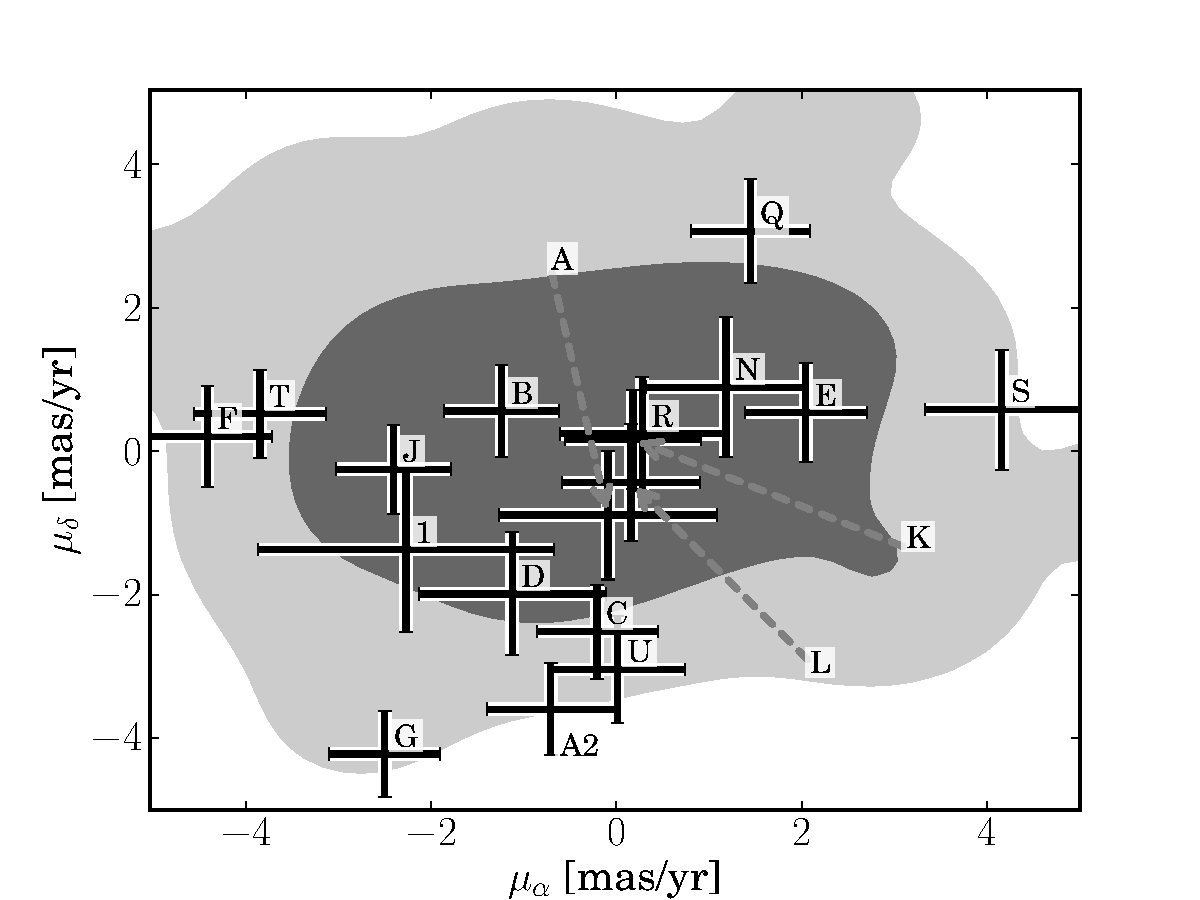
\includegraphics[width=0.5\textwidth]{chapter_sn1572_hires/plots/propmot_distr.pdf}
   \caption[Proper motion measurement of stars in SN 1572 using only HST images]{The contours show the distribution of proper motion ($1-\sigma$ and $2-\sigma$) excluding the named stars.
    We show the location of the candidate stars and their errors on top of this distribution. Tycho-2 was not shown in this figure as it is an extreme outlier with $\mu_\alpha=75$~\masyr\ and $\mu_\delta=-4.4$~\masyr\ but also at a large distance to the center of the remnant's geometric center (46\arcsec).}
   \label{fig:propmot_sn1572_hires}
\end{figure}


\subsection{Radial Velocity}
\label{sec:radvel}

The radial velocity of each star was measured using the IRAF task \textit{fxcor} \citep{1979AJ.....84.1511T}. MAKEE was used to calculate an intrinsic velocity shift by comparing offsets of the nightsky-lines. The radial velocity standards were reduced in the same fashion. 
 
Each order of each star was then cross-correlated with at least two other radial velocity standards (\object{HR6349}, \object{HR6970} \& \object{HR1283}) which had been observed on the same night.


The radial velocity for \starb\ was measured in the course of determining the stellar parameters for \starb\ with the stellar parameter fitting package \gls{sfit}. The \gls{sfit} result consistently gives $v_\textrm{helio} = -55~\kms$ for different stellar parameters with an error of $\approx 2~\kms$. 


In Table \ref{tab:radvel} we have listed all the radial velocities both in a heliocentric frame and a local-standard-of-rest (henceforth LSR) frame. We will be referring to the heliocentric measurements from here on. The listed error is the standard deviation of the radial velocity measurement of all orders added in quadrature to the error of the radial velocity standards.

In Figure \ref{fig:dist_vr} we have compared the radial velocity of our sample stars to radial velocities of stars in the direction of Tycho's SNR using the Besan\c{c}on Model \citep{2003A&A...409..523R}. The distance as well as the error in distance are taken from Section \ref{sec:distance}.  The candidates radial velocities are all typical for their distance. Finally, we note the measurement of \starg\ is consistent with \wek\ and \gh.

\ctable[
caption = {Radial velocities},
label = {tab:radvel},
]
{lccccc}{}{\FL
Name & Date & $v_\textrm{helio}$ & $v_\textrm{LSR}$ &$\Delta v$ \\
designation & (dd/mm/yy) & (\kms) & (\kms) & (\kms) \ML
%startdata
\stara & 09/09/06 & -36.79 & -28.5 & 0.23   \\
\starb & 09/09/06 & -55.0 & -57.0 & $\approx 2$ \\
\starc & 11/10/06 & -58.78 & -50.49 & 0.75   \\
\stard & 11/10/06 & -58.93 & -50.64 & 0.78   \\
\stare & 11/10/06 & -64.2 & -55.91 & 0.27   \\
\starg & 09/09/06 & -87.12 & -78.83 & 0.25 \\
\starg & 11/10/06 & -87.51 & -79.22 & 0.78 
\LL
}

\begin{figure}[htbp] %  figure placement: here, top, bottom, or page
   \centering
   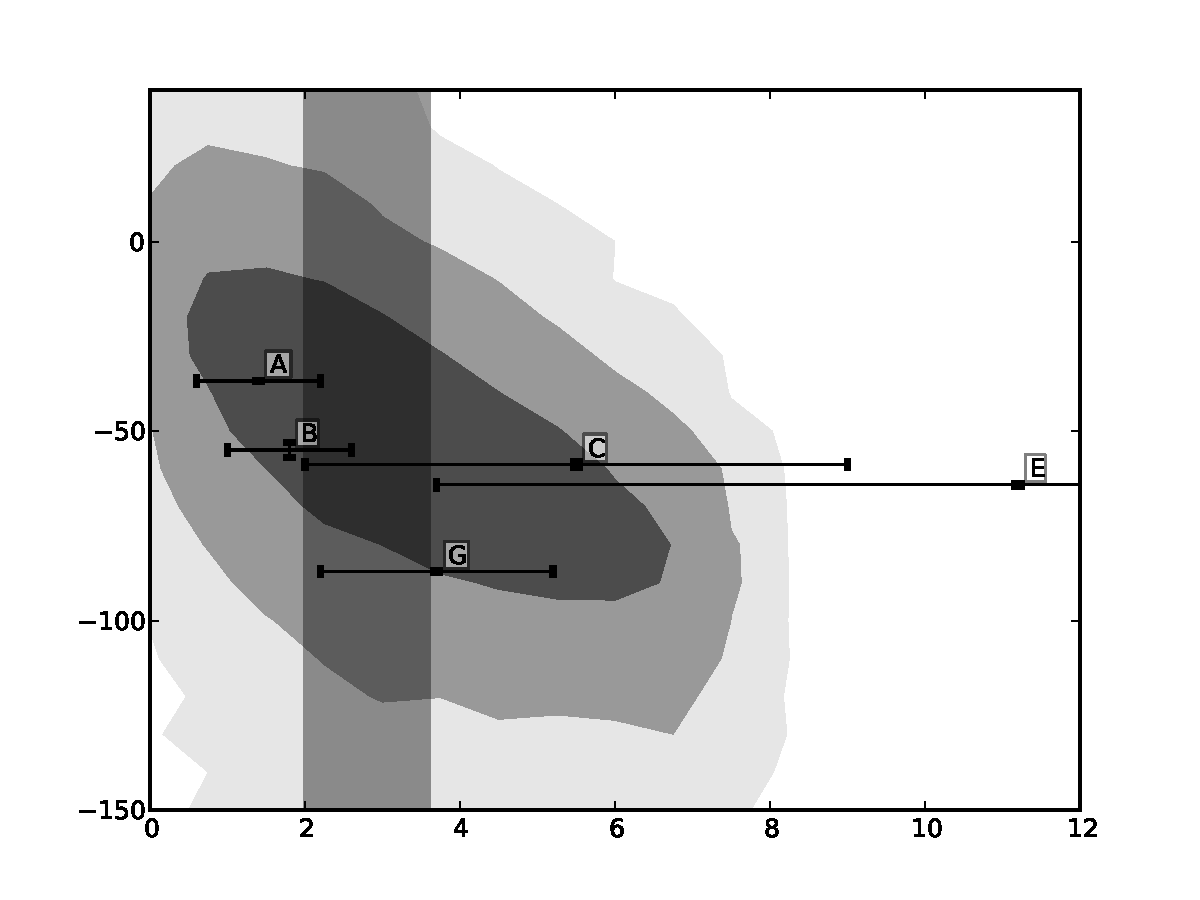
\includegraphics[width=0.5\textwidth]{chapter_sn1572_hires/plots/dist_vr.pdf} 
   \caption[Radial velocity of all candidate stars in SN 1572 with the Besan\c{c}on Model]{The contours indicate 1, 2 and $3-\sigma$ levels of the distance and radial velocity using the Besan\c{c}on Model \citep{2003A&A...409..523R} with $\approx 60 000$ stars in the direction of SNR1572 (only including star with a V between 10 and 20 as well as stars with a metallicity of [Fe/H] $> -1$). We have overplotted our candidate stars with error bars. One should note that the errors in distance are only an indication of the error, the proper error surfaces can be seen in Figure \ref{fig:mc_isochrone}. The vertical gray shade shows the error range for the distance of SNR1572.}
   \label{fig:dist_vr}
\end{figure}



\subsection{Rotational Velocity}
\label{sec:rotation}
We have measured rotational velocities of all stars except \starb\ in the same fashion as described in \wek. We selected several unblended and strong (but not saturated) \ion{Fe}{1} lines in the stellar spectra .  We added these lines after shifting them to the same wavelength and scaling them to the same \gls{ew}. This was done to improve the signal to noise ratio for the faint stars as well as providing consistency throughout all stars. 

 As a reference we created three synthetic spectra for each star (one broadened only with the instrumental profile, the others with the instrumental profile and $\vrot\sin{i}$\ of 10 and 13~\kms\ respectively) with the 2010 version of \gls{moog}, using our derived temperature, gravity and metallicity.  As input data to \gls{moog} we used the \citet{2004astro.ph..5087C} atmospheric models and a line list from \citet{1995KurCD..23.....K}. We then applied the same process of line selection and adding as for the lines in the observed spectra. 
 
Figure \ref{fig:sn1572_hires:rotvel} shows the comparison between the synthetic spectra of different rotational velocity and the observed spectra. This comparison indicates that the stellar broadening (rotational, macro turbulence, etc. ) is less than broadening due to the instrumental profile of 6~\kms\ for each star. We adopt 6~\kms\ as an upper limit to the rotation for all stars.



\begin{figure}[h!]
\begin{tabular}{cc}
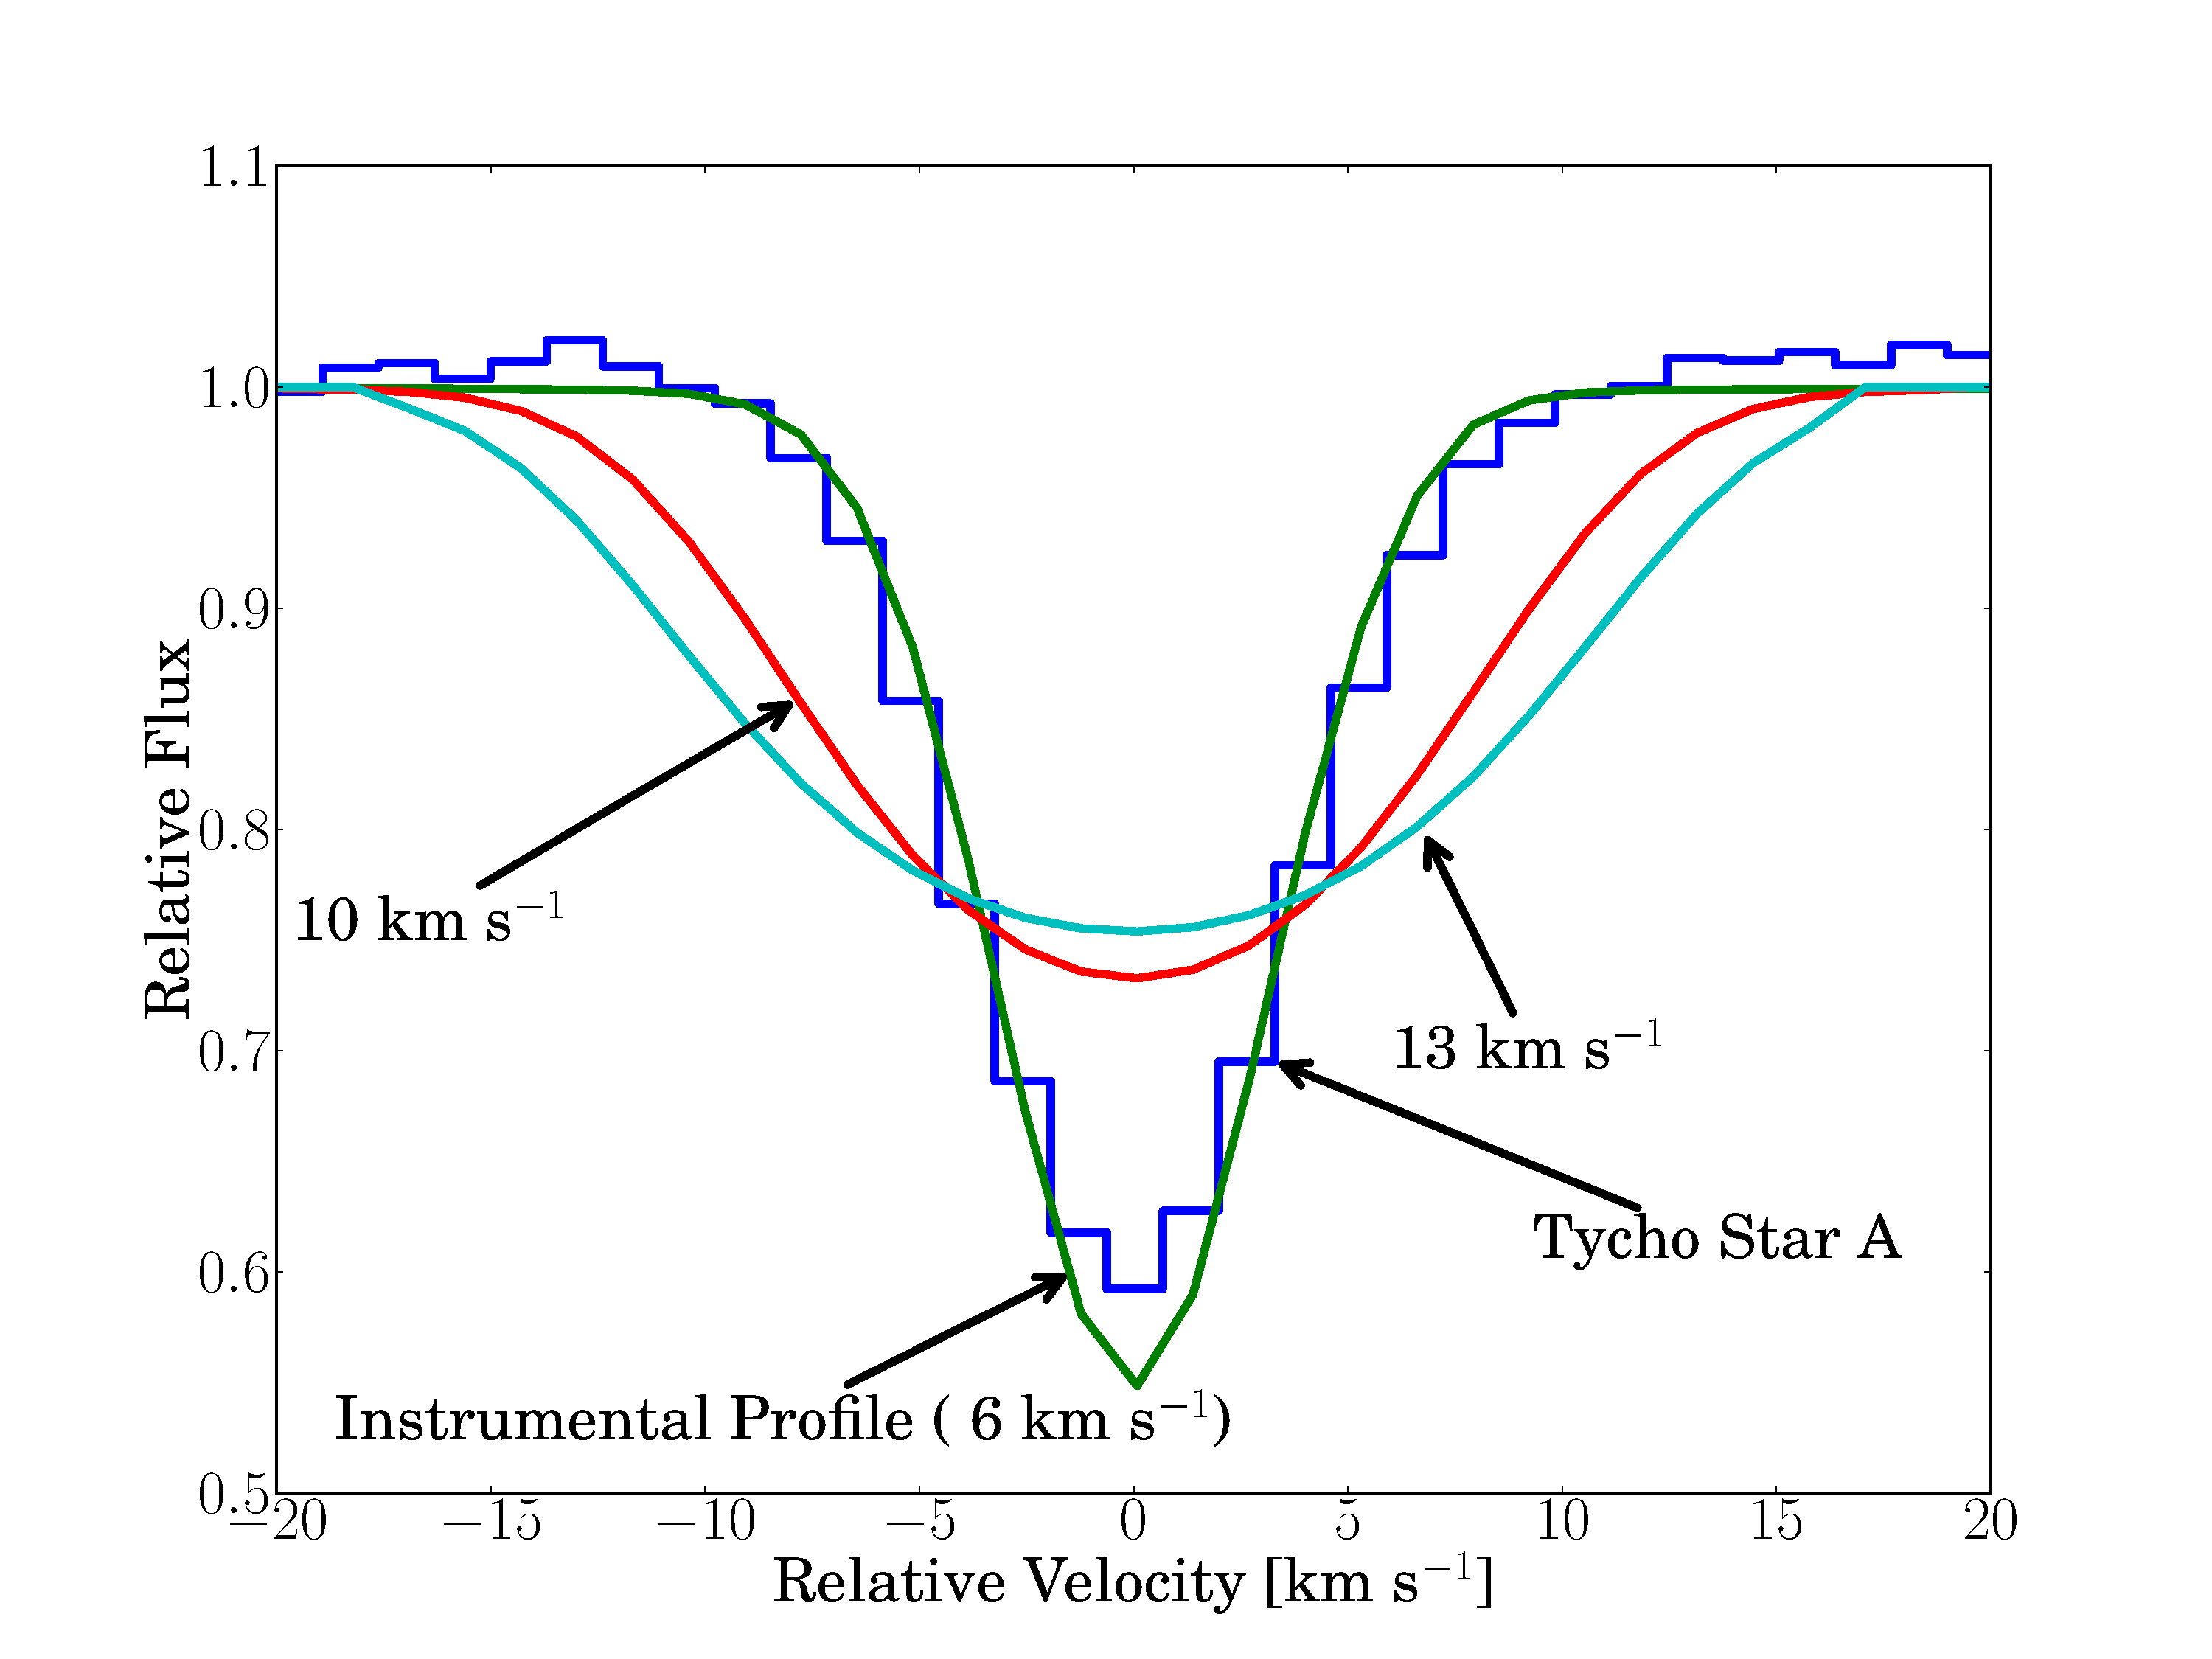
\includegraphics[width=0.45\textwidth, trim=130 30 60 0]{chapter_sn1572_hires/plots/stara_rotation.pdf} &
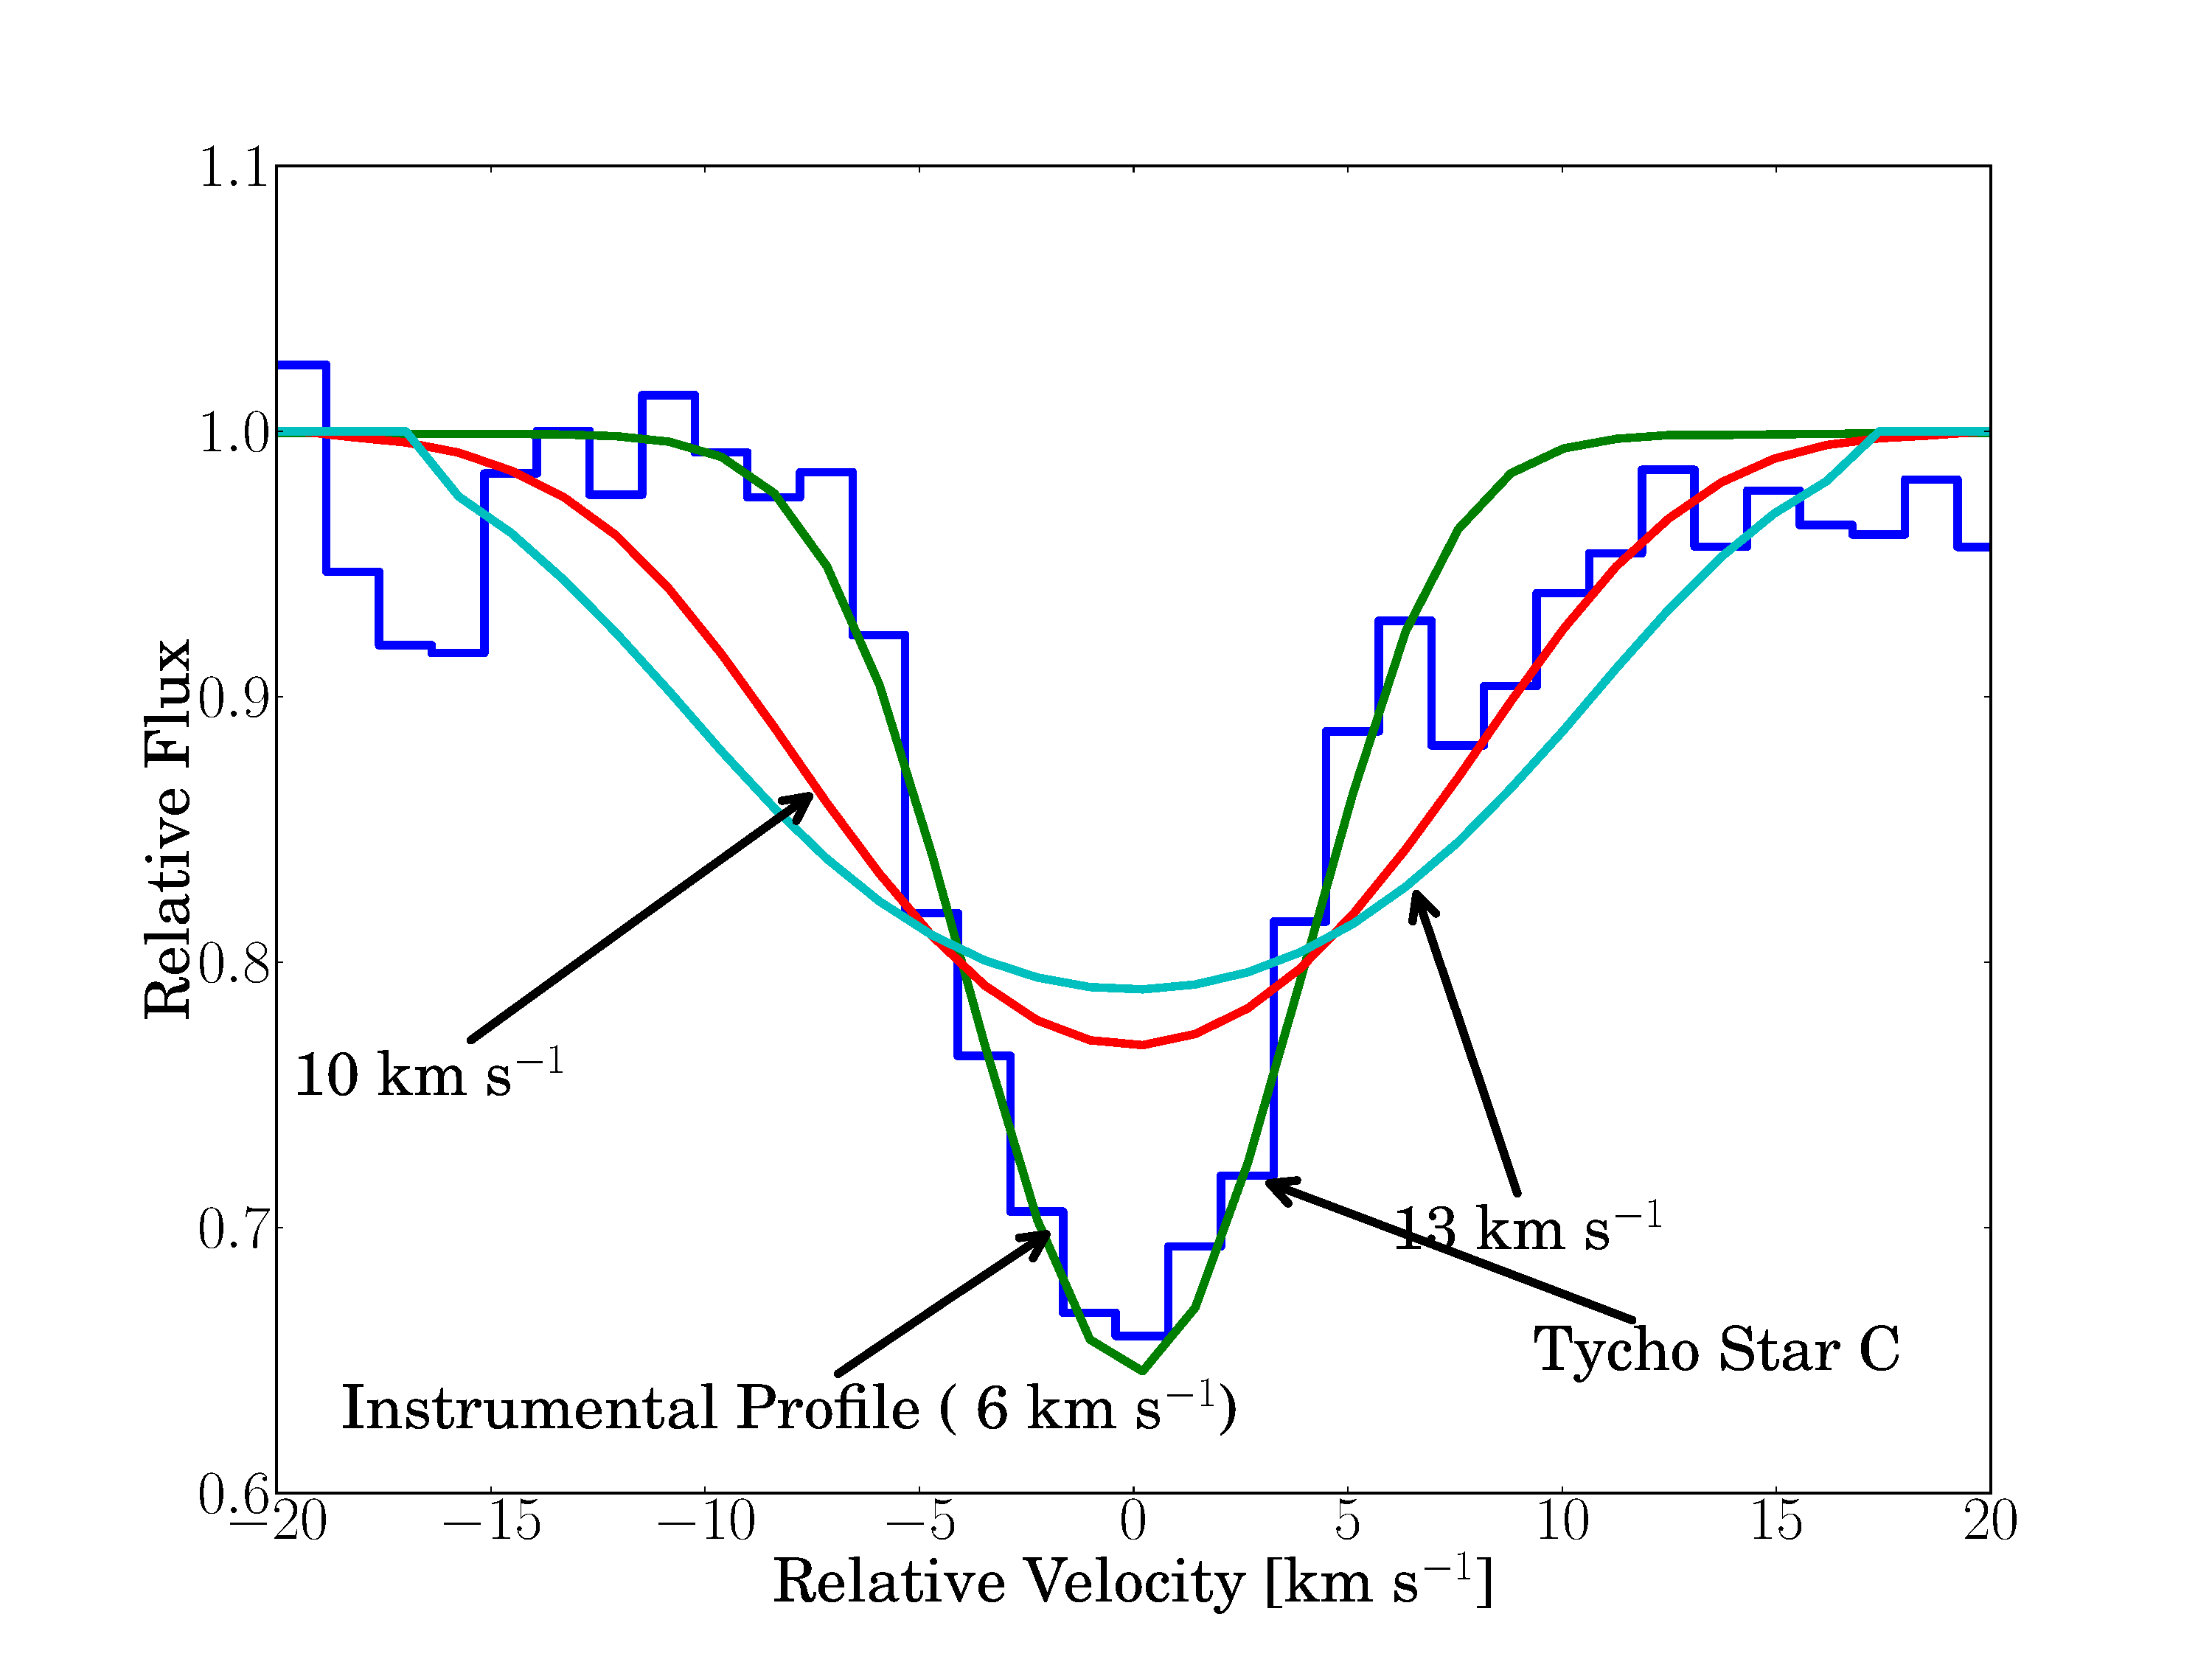
\includegraphics[width=0.45\textwidth, trim=130 30 60 0]{chapter_sn1572_hires/plots/starc_rotation.pdf} \\
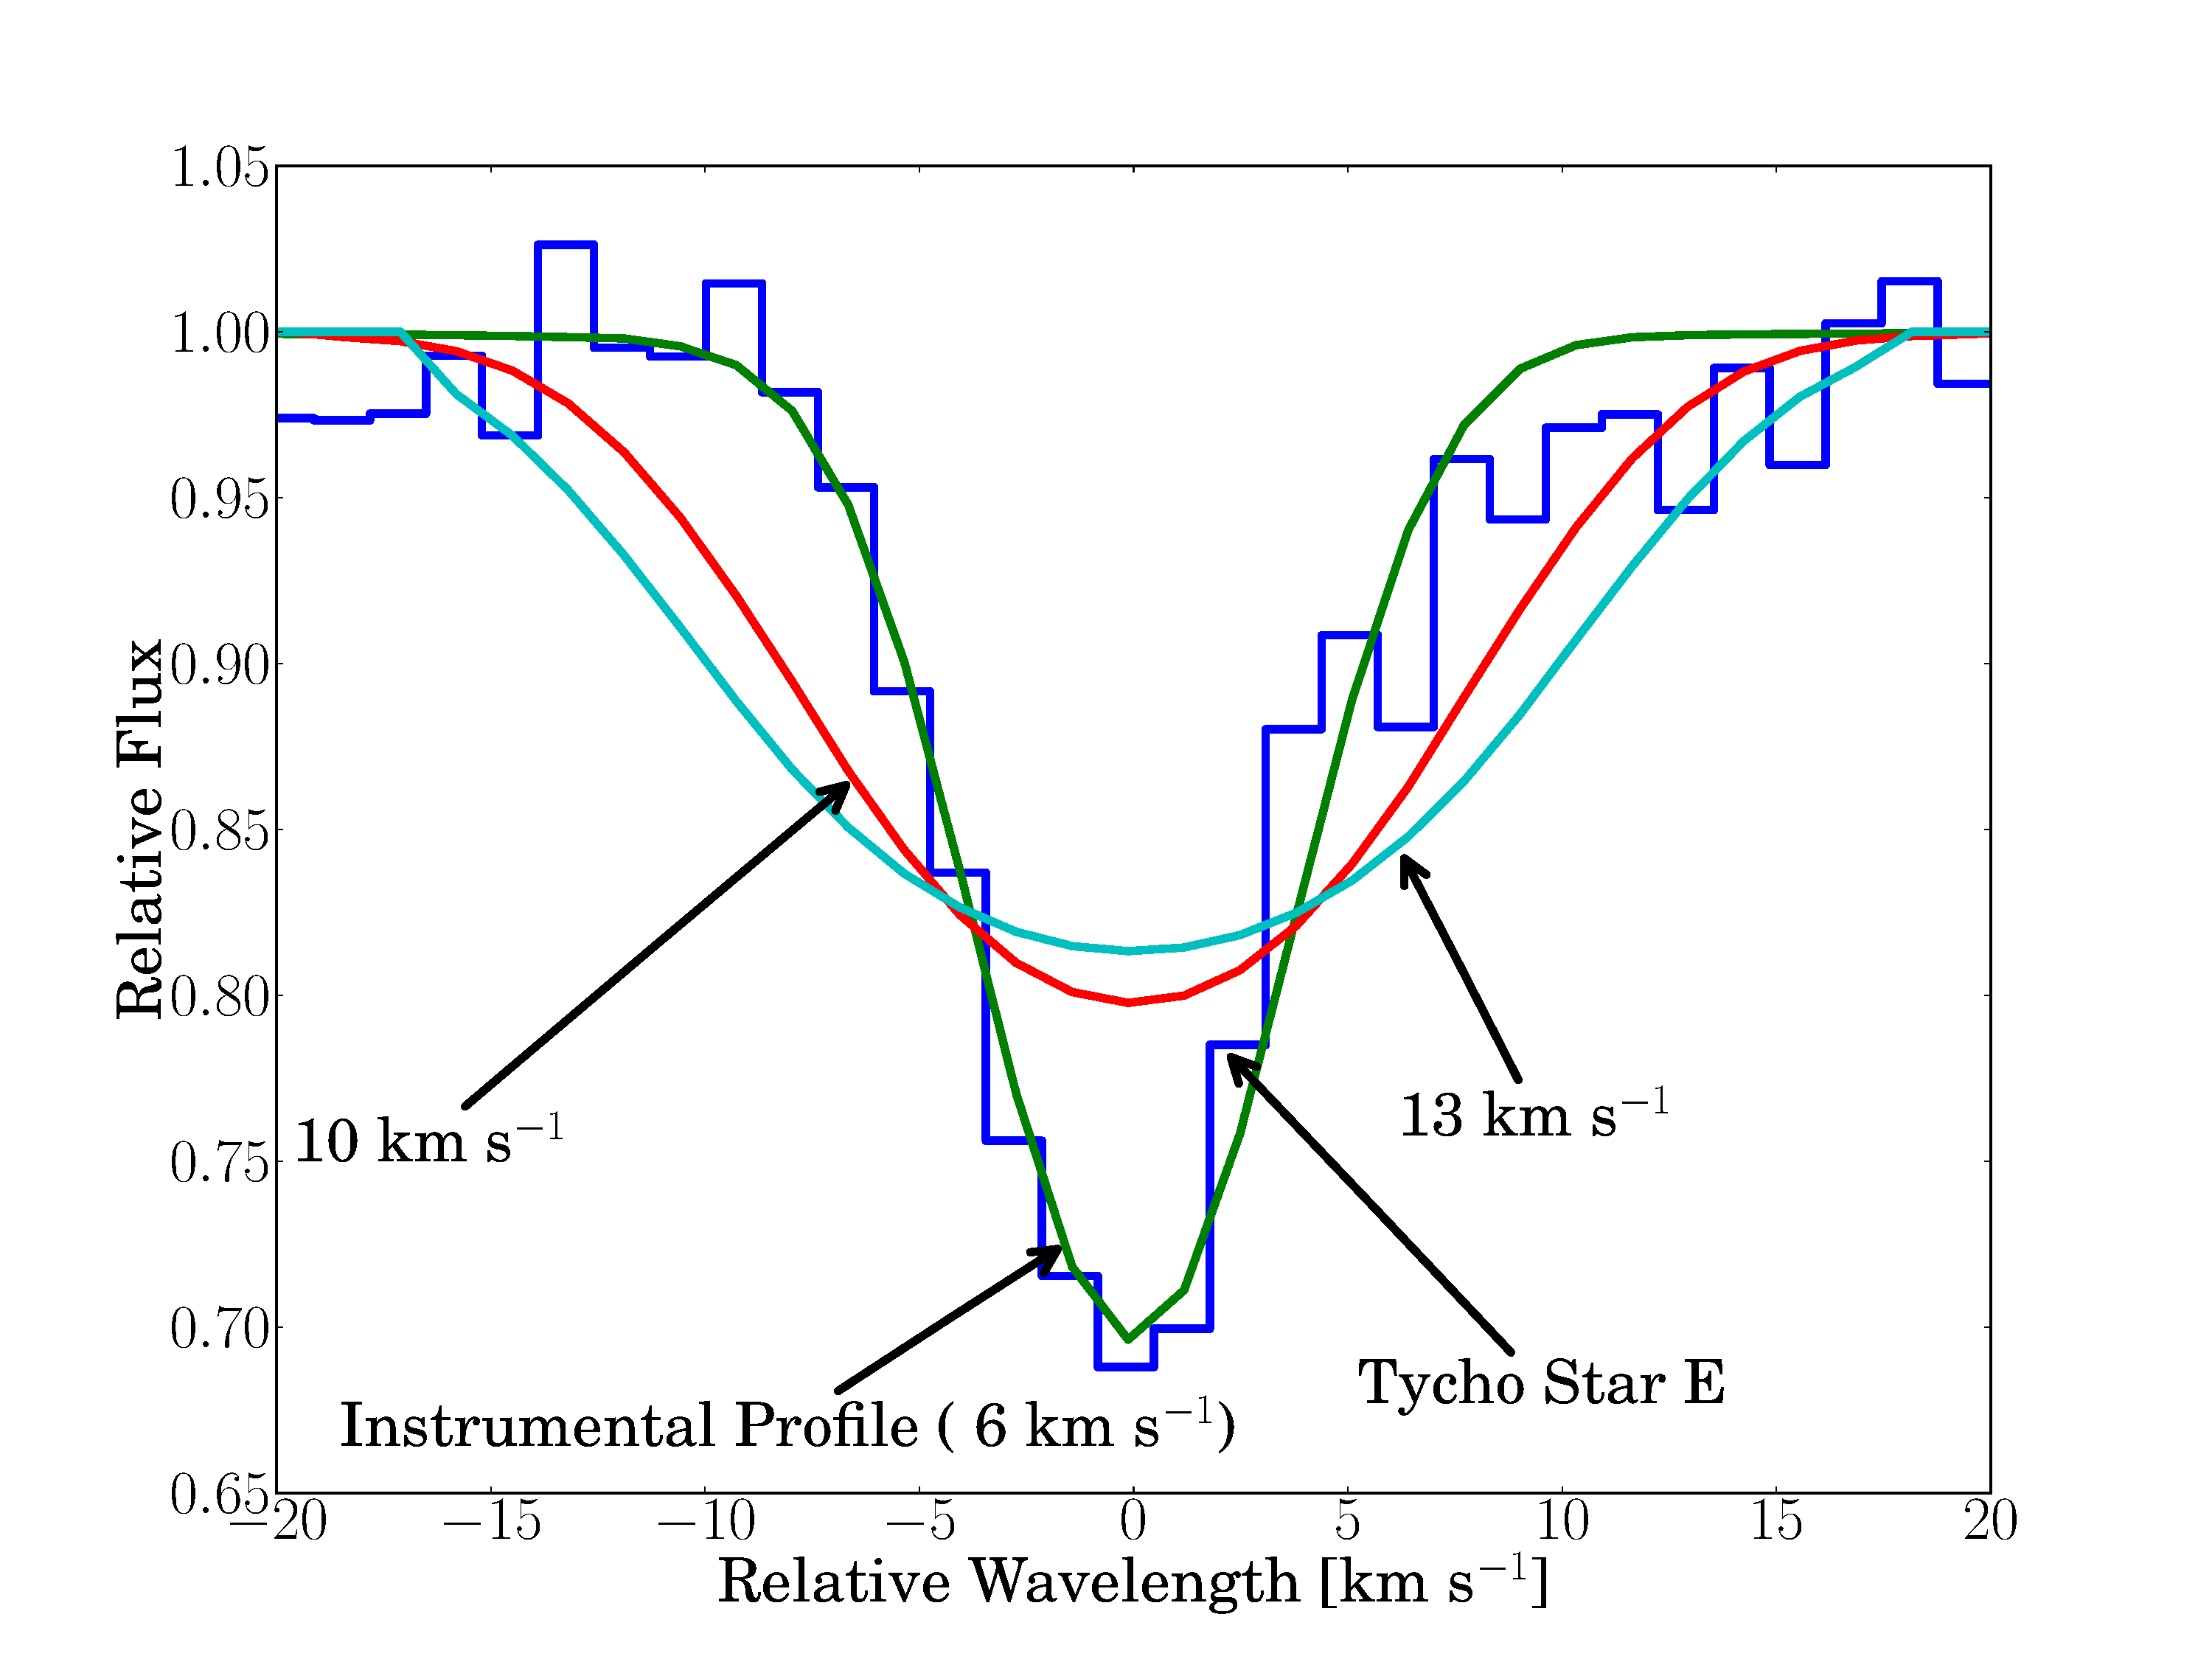
\includegraphics[width=0.45\textwidth, trim=130 30 60 0]{chapter_sn1572_hires/plots/stare_rotation.pdf} &
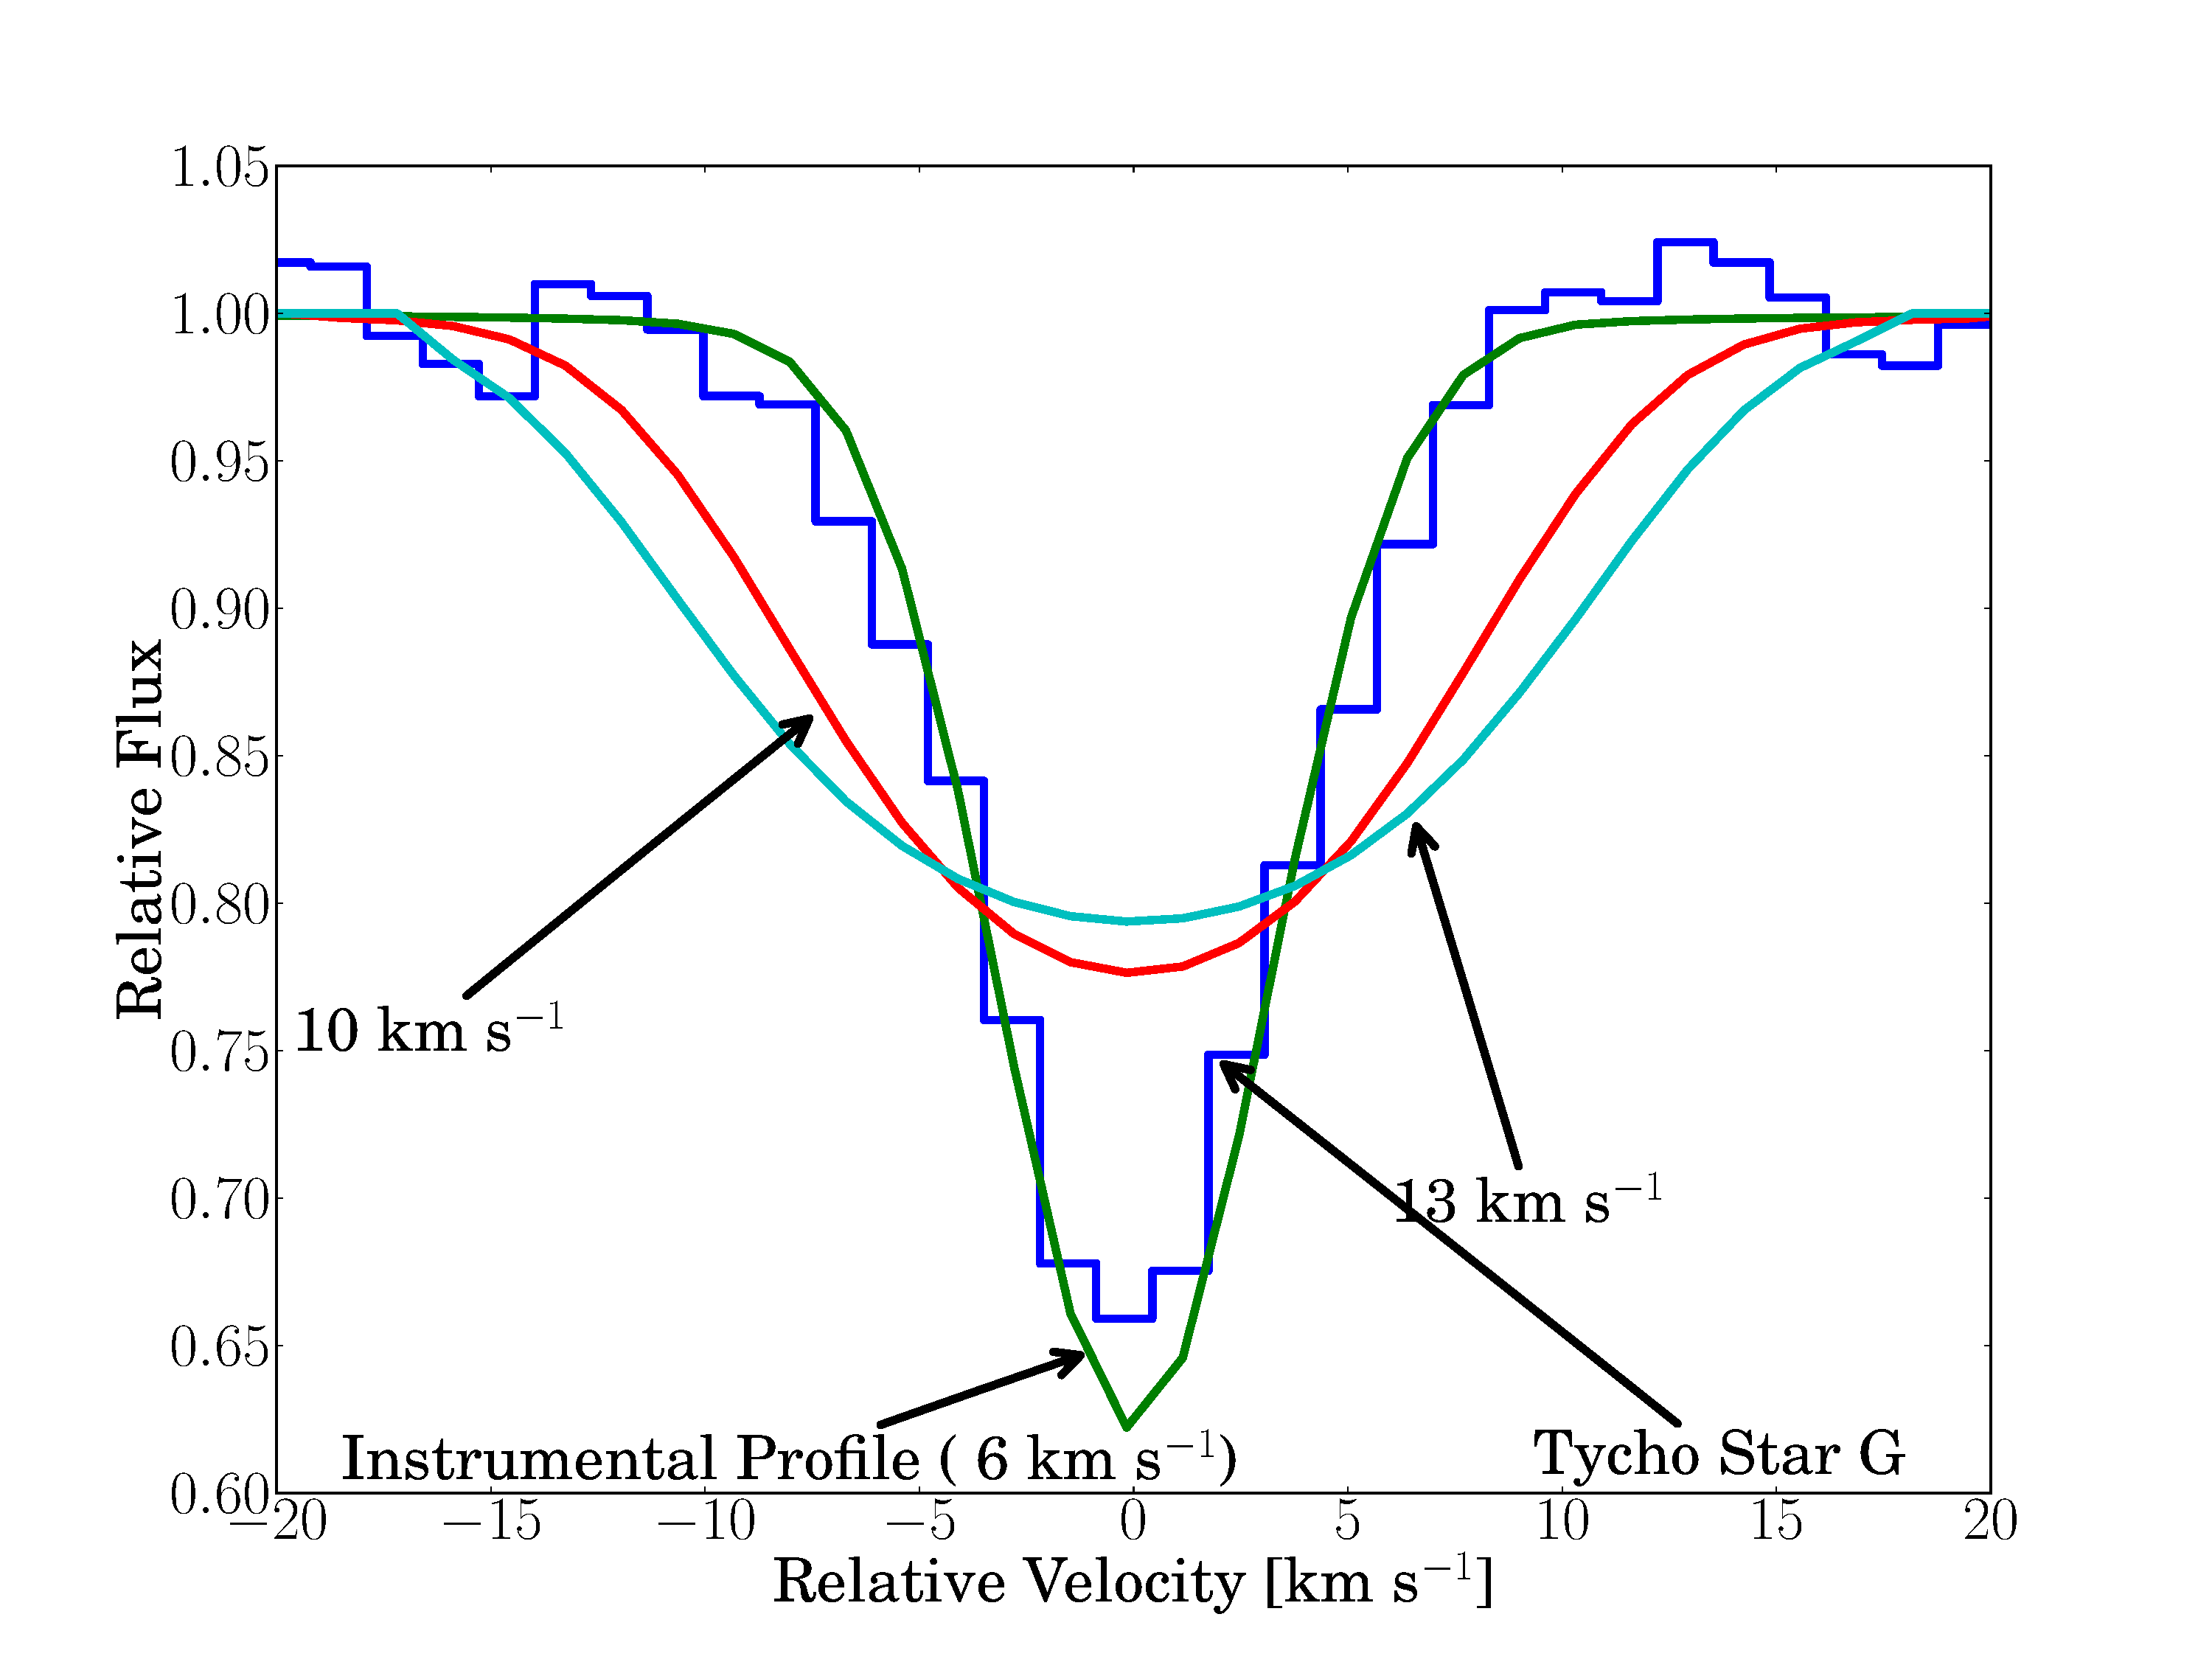
\includegraphics[width=0.45\textwidth, trim=130 30 60 0]{chapter_sn1572_hires/plots/starg_rotation.pdf} \\
\end{tabular}
\caption[Rotation measurement for all candidate stars in SN 1572]{The figures show the combination of iron line profiles after normalization to the same \glsentryname{ew} and compare them to synthetic line profiles created by \glsentryname{moog}. We convolved the synthetic lines first with a rotational kernel with three different values for rotation and then with the instrumental profile. All stars show rotation less than 6~\kms\ which is equal to the instrumental profile at this resolution. }
\label{fig:sn1572_hires:rotvel}
\end{figure}

Due to its high temperature and rotation, we fit the rotational velocity for \starb\ with the program \gls{sfit} \citep[][described in section \ref{sec:stellar-parameters}]{2001A&A...376..497J}  as part of the overall fit for this star's stellar parameters.  We find $\vrot=171^{+16}_{-33}$~\kms. While \starb's rotation is very high compared to the other candidate stars,  for stars of this temperature and gravity a high rotation is not unusual. In summary, none of the stars show rotation which is measurable at this resolution.


\subsection{Stellar parameters}
\label{sec:stellar-parameters}
The stellar parameters are presented in Table \ref{tab:sn1572_hires:stel_param} and were determined using a traditional spectroscopic approach based on the \glspl{ew} of lines of different excitation and ionization levels. . These measurements exclude \starb, due to its hot temperature, and we measure its stellar parameters by direct comparison to models, in a separate procedure.

\glspl{ew} for a set of Fe lines were measured using routines in IRAF (compiled from \citet[][henceforth Reddy03]{2003MNRAS.340..304R} and \citet[][henceforth RC02]{2002AJ....123.3277R} Table \ref{tab:sn1572_hires:llist} shows the \glspl{ew} measured for each of the stars. Missing values indicate that the line was not detected. 

We used the local thermodynamic equilibrium (LTE) stellar line analysis program MOOG \citemoog\ and LTE model atmospheres from the \citet{2003IAUS..210P.A20C} grid to derive an abundance for a given line. The \gls{teff} was adjusted until the abundances from \ion{Fe}{1} lines displayed no trend as a function of excitation potential. The \gls{logg} was adjusted until the abundances from \ion{Fe}{1} and \ion{Fe}{2} lines were in agreement. The microturbulent velocity, $\xi _{t}$ , was adjusted until there was no trend between the abundances from the \ion{Fe}{1} lines and EW. This process was iterated until self consistent stellar parameters were obtained  for each star. In our analysis, we explored stellar parameters at discrete values. For \gls{teff}, we considered values at every 25 K (e.g. 4000, 4025 K, etc.), for \gls{logg} , we considered values at every 0.05 dex (e.g., 1.00, 1.05 dex, etc.), and for $\xi _{t}$ , we considered values at every 0.05~\kms (e.g. 1.70, 1.75~\kms, etc.). We assumed that excitation equilibrium was satisfied when the slope between $\log{\epsilon}$(\ion{Fe}{1}) and lower excitation potential $(\chi)$ was $\leq0.004$. We assumed that ionization equilibrium was achieved when $\vert\log{\epsilon} ($\ion{Fe}{1}$) - \log{\epsilon} ($\ion{Fe}{2}$)\vert \leq 0.02$~dex. The microturbulent velocity was set when the slope between $\log{\epsilon}$(\ion{Fe}{1}) and reduced \gls{ew} ($\log{\textrm{W}}/\lambda$) was $\leq0.004$. In all cases we found appropriate solutions in which the trends between \ion{Fe}{1}, \ion{Fe}{2}, \glspl{ew} and excitation potentials were small. We estimate that the internal errors are typically $\glssymbol{teff}, \pm100$~K, $\log{g}\pm0.3$~dex, and $\xi _{t}\pm0.3$~\kms. For further details regarding the derivation of stellar parameters, see \citet{2008ApJ...673..854Y}.

The final iron measurements are the average of \ion{Fe}{1} and \ion{Fe}{2} assuming the solar abundances of \citet{2009ARA&A..47..481A} 
In addition, we measured abundance for the Elements nickel and lithium via \gls{ew} analysis. We could not see any unusual abundance pattern for any of the sample stars (see Figure \ref{fig:kobayashi06}; \starb's abundances are not presented on the plot as they were measured in a different fashion).  


\ctable[
caption = {Stellar Parameters},
label = {tab:sn1572_hires:stel_param}
]
{lccccccc}{}{\FL
Name & \teff & \logg & \feh & $\Delta$\gls{feh}& [Ni/H] & $\Delta$[Ni/H] & [Li/H] \\ 
designation & (K) & (dex) & (dex) & (dex) & (dex) & (dex) & (dex) \ML 
%\startdata
\stara & 4975 & 2.9 & 0.02 & 0.16 & 0.05 & 0.025 & 0.09 \\
\starc & 4950 & 2.9 & -0.57 & 0.23 & -0.14 & -0.17 & 0.11 \\
\stare & 5825 & 3.4 & -0.16 & 0.21 & 0.2 & 0.0 & 0.131\\
\starg & 6025 & 4 & -0.15 & 0.18 & 0.14 & 0.08 & 0.11 \LL
}

\ctable[
width=\textwidth,
caption = {Measured \glsentryplural{ew} from the Keck HIRES spectra},
label = {fig:sn1572_hires:llist},
]
{lccccccc}{}{\FL
$\lambda$ & $\chi$ & $\log{gf}$ & Source & \stara & \starg & \starc & \stare \\ 
(\AA) & (eV) & (dex) & & (dex) & (dex)& (dex) & (dex) \ML
%
%\startdata
5082.35 & 3.658 & -0.59 & Reddy03 & 6.31 & 6.44 &   & 6.2 \\
5088.54 & 3.85 & -1.04 & Reddy03 & 6.19 & 6.33 &   &   \\
5088.96 & 3.68 & -1.24 & Reddy03 & 6.21 &   &   &   \\
5094.42 & 3.83 & -1.07 & Reddy03 & 6.1 &   &   &   \\
5115.4 & 3.834 & -0.28 & Reddy03 & 6.22 &   &   &   \\
5682.20 & 4.10 & -0.47 & RC02 & 6.34 &   &   &   \\
5748.351 & 1.68 & -3.26 & RC02 & 6.33 &   & 5.74 &   \\
5749.297 & 3.94 & -1.99 & RC02 & 6.38 &   &   &   \\
5847.01 & 1.676 & -3.41 & Reddy03 & 6.26 &   & 5.55 &   \\
6007.31 & 1.68 & -3.34 & RC02 & 6.2 &   & 5.45 &   \\
6053.685 & 4.23 & -1.07 & RC02 & 6.33 &   &   &   \\
6086.28 & 4.26 & -0.52 & RC02 & 6.25 & 6.22 &   &   \\
6108.116 & 1.68 & -2.44 & RC02 & 6.26 & 6.11 & 5.33 &   \\
6111.08 & 4.088 & -0.81 & Reddy03 & 6.33 &   & 5.38 &   \\
6130.14 & 4.266 & -0.94 & Reddy03 & 6.31 &   &   &   \\
6175.37 & 4.089 & -0.55 & Reddy03 & 6.25 & 6.35 & 5.7 &   \\
6176.82 & 4.09 & -0.26 & Reddy03 & 6.3 & 6.27 & 5.43 & 6.01 \\
6177.25 & 1.83 & -3.51 & Reddy03 & 6.23 &   &   &   \\
6186.71 & 4.10 & -0.97 & RC02 & 6.33 & 6.23 &   &   \\
6204.61 & 4.09 & -1.11 & Reddy03 & 6.32 &   &   &   \\
6322.17 & 4.15 & -1.17 & RC02 & 6.31 &   &   &   \\
6370.346 & 3.54 & -1.94 & RC02 & 6.37 &   &   &   \\
6378.26 & 4.154 & -0.83 & Reddy03 & 6.3 &   & 5.81 &   \\
6482.80 & 1.93 & -2.63 & RC02 & 6.2 &   & 5.38 &   \\
6598.60 & 4.23 & -0.98 & RC02 & 6.3 &   & 5.74 &   \\
6635.12 & 4.42 & -0.83 & RC02 & 6.37 &   &   &   \\
%\tablebreak
6643.64 & 1.68 & -2.03 & Reddy03 & 6.48 & 6.02 & 5.34 & 5.97 \\
6767.772 & 1.83 & -2.17 & RC02 & 6.35 & 6.19 & 5.67 &   \\
6772.32 & 3.658 & -0.97 & Reddy03 & 6.31 &   &   &   \\
6842.037 & 3.66 & -1.47 & RC02 & 6.4 & 6.36 &   &   \\
7030.011 & 3.54 & -1.73 & RC02 & 6.42 &   &   &   \\
7122.197 & 3.54 & 0.048 & RC02 & 6.33 &   & 5.34 &   \\
7261.918 & 1.95 & -2.7 & RC02 &   & 6.26 &   &   \\
7327.648 & 3.8 & -1.77 & RC02 & 6.38 & 6.44 &   &   \\
7409.35 & 3.8 & -0.1 & RC02 &   &   & 5.24 &   \\
7414.502 & 1.99 & -2.57 & RC02 &   & 6.2 & 5.57 & 6.03 \\
7422.275 & 3.63 & -0.129 & RC02 & 6.47 &   & 5.32 & 5.84 \\
7574.048 & 3.83 & -0.58 & RC02 & 6.3 & 5.97 & 5.12 &   \\
7748.89 & 3.7 & -0.38 & Reddy03 & 6.42 & 6.17 & 5.41 & 6.27 \\
7788.93 & 1.95 & -2.42 & RC02 &   &   & 5.87 & 6.33 \\
7797.59 & 3.9 & -0.35 & Reddy03 & 6.41 & 6.16 & 5.59 & 6.2 \\
7917.44 & 3.74 & -1.5 & RC02 &   & 6.14 &   &   \LL
}

\begin{figure}[h] %  figure placement: here, top, bottom, or page
   \centering
   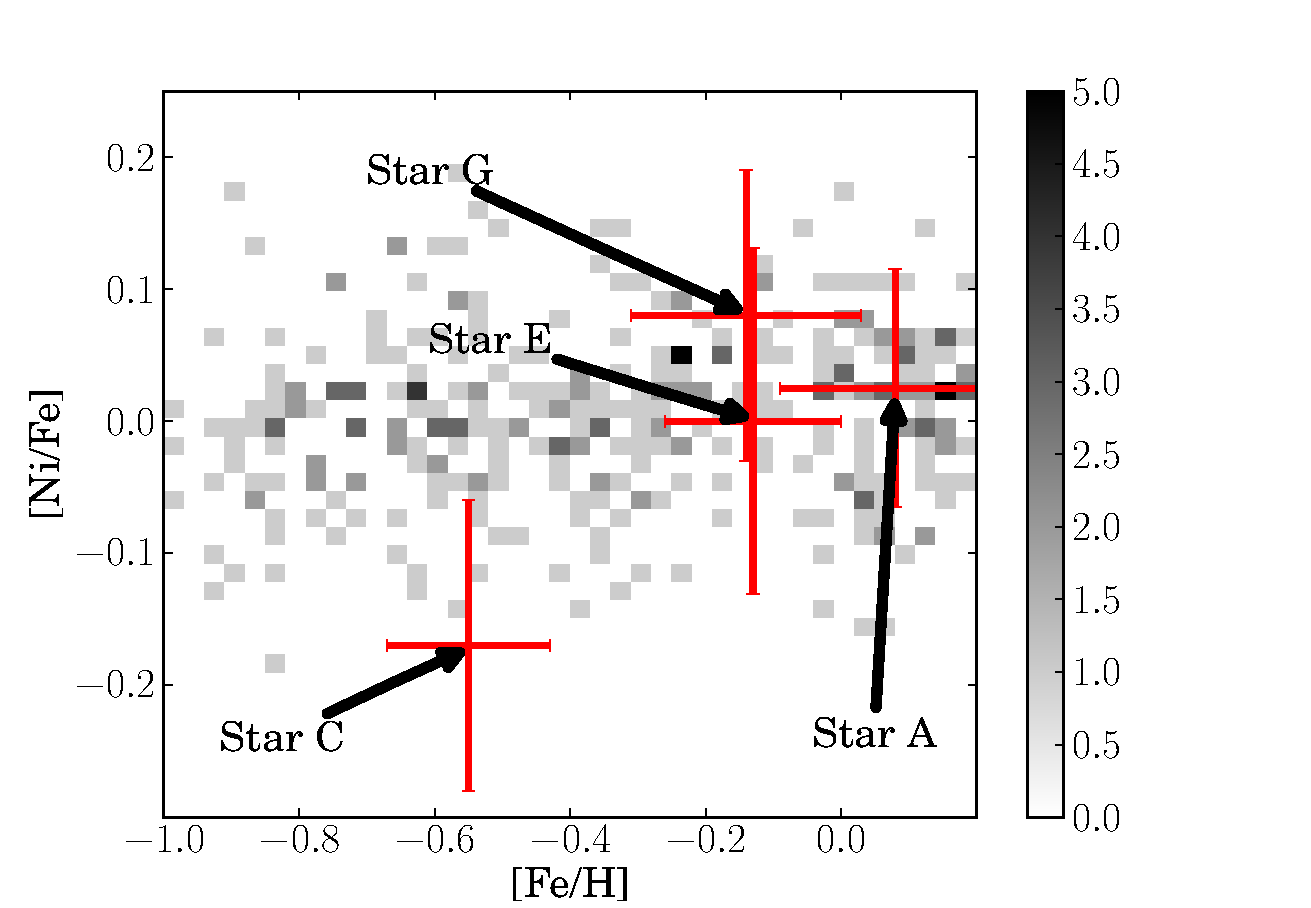
\includegraphics[width=1\textwidth]{chapter_sn1572_hires/plots/abund_chiaki.pdf} 
   \caption[Comparison of nickel and iron abundance measurement of stars in SN 1572]{The background colour indicates the distribution is taken from \citet{2006ApJ...653.1145K}. All of the measured candidates are consistent within the errors with stars of the same metallicity.}
   \label{fig:kobayashi06}
\end{figure}

In summary, the inferred metallicities for all candidates show that the candidates are of roughly solar metallicities with the exception of the metal-poor \starc. The range of metallicities spanned by the program stars is compatible with membership of the thin disk. Based on metallicity alone, we do not regard any of the program stars to be unusually metal-poor or metal-rich.  Additionally, we find the [Ni/Fe] abundance to be consistent with stars of similar metallicity (see Figure \ref{fig:kobayashi06}). The stellar paramaters and elemental abundances are listed in Table \ref{tab:stel_param}.

Because \starb\ has a temperature  greater than 9000\,K and is quickly rotating, the process described above cannot be used to measure stellar parameters. Instead we used the program \gls{sfit} to match the \gls{hires} spectrum to a grid of model spectra. To determine the stellar parameters for \starb\ we have used a model grid with $\feh= -1.0$, $8000 < \teff < 16000$, $7 < \log{g} < 2$. This low metallicity is suggested by a very weak Calcium K line and Mg II lines, but is hard to measure. We can not measure Helium directly in this spectrum and thus adopt N(He) = 0.1 as this is empirically a very common Helium abundance in stars.

This analysis resulted in $\teff = 10000^{+ 400}_{-200}~\textrm{K}$, $\log{g} = 3.67$ with slope  $\partial \logg/\partial \teff = 0.27/500~\textrm{K}^{-1}$, rotational velocity $\vrot \sin{i} = 171$\,\kms\ with slope $\partial \vrot \sin{i} / \partial \teff =$ $ -41/500\,\kms\,\textrm{K}^{-1}$. From qualitative analysis this object seems metal poor (e.g. in comparison to stars of similar stellar parameters but solar metallicity), but its high rotation and temperature make it hard to determine this parameter precisely. For the present, we assume [Fe/H] = -1.0 unless otherwise noted.

In addition, using the high-resolution spectrum, we measured the \glspl{ew} of several lines predicted to be strong in the VALD database \citep{2000BaltA...9..590K}. The abundances were deduced from the \glspl{ew} using a model atmosphere having $T_{\textrm eff} = 10000$\,K, $\log{g}=3.67$ and [Fe/H] = -1.0 (see Table \ref{tab:starb-abund}).

One caveat regarding these abundances is the use of \glspl{ew} from 
single lines with large rotational broadening, since the effect of blending 
with nearby weak lines cannot be taken into account. A second is that these 
abundances invariably rely on the strongest lines, which are precisely those 
most susceptible to departures from local thermodynamic equilibrium. 
Nevertheless, they do confirm the earlier impression that the star is 
metal-poor, and justify the adoption of \feh=$-1.0 \pm 0.4$.


\ctable[
caption={\starb\ abundances},
label={tab:starb-abund},
]
{lcccccc}{}{\FL
Ion&$\lambda$& $W_{\lambda}$& $\epsilon$& $[X/H]$ & $\frac{\partial \epsilon}{\partial \logg}$  &$\frac{\partial \epsilon}{\partial \teff}$\\
designation & \AA & \AA & dex & dex& &K$^-1$ \ML
%\startdata
\ion{Mg}{2} & 4481.13+4481.33 & $220\pm15$ & $6.18\pm.08$ & -1.40&0.08&$8\times10^{-5}$ \\ 
\ion{Si}{2} & 6347.1 & $140\pm5$ & $6.96\pm.18$ & -0.59&-0.02&$1\times10^{-4}$\\
\ion{O}{1} & 7771.9+7774.2+7775.4 & $460\pm30$ & $8.43\pm.10$ & -0.58 &0.24&$-4\times10^{-5}$ \LL
}


As a second approach to determine the stellar parameters of \starb\ we used the low resolution spectra observed with LRIS.  The observation range of LRIS was chosen to be centered around the Balmer jump as this feature is sensitive to the surface gravity \citep{2007PASP..119..605B}. We fitted the spectra to a grid of model spectra \citep[]{2005A&A...442.1127M} using a spectrum fitting tool  described below. The final grid we used covered $\log{g}$ from 3.5 to 4.5 in steps of 0.5 and \gls{teff} from 9000 to 12000\,K in steps of 500\,K. In addition we expanded the grid by reddening the spectra with the \textit{pysynphot}-package\footnote{pysynphot is a product of the Space Telescope Science Institute, which is operated by AURA for NASA.}. We also added diffuse interstellar bands  \citep{1937PASP...49..224B, 1966ZA.....64..512H, 1967IAUS...31...85H, 1975ApJ...196..129H, 1995ARA&A..33...19H, 1994dib..nasa...31H, 1994A&AS..106...39J, 1958ApJ...128...57W} to the synthetic spectra , which were scaled with reddening . The included E(B-V) ranged from 0.5 to 1.3 in steps of 0.2. We assumed a rotation of 171\,\kms\ in the grid  (see section \ref{sec:rotation}).

We used $\chi^2$ as a figure of merit in our fitting procedure. To find the best fit for \starb\ we used the \gls{migrad} algorithm provided by \gls{minuit} and linearly interpolated between the grid points using \textsc{LinearNDInterpolator} provided by the \gls{scipy}. The fit of \starb\ results in \glssymbol{teff}=10570\,\textrm{K}, \logg=4.05, \feh=-1.1 and E(B-V)=0.85. The model fits the synthetic spectrum poorly  in the wavelength region between 3800 -- 4280 \AA\ in (see Figure \ref{fig:starb_spec_comp}). The adopted mixing length parameter used in 1D model atmospheres, used to construct the spectral grid, influences the fluxes in that region as well as affecting the hydrogen line profiles. \citet{2002A&A...392..619H} and others show that a mixing length of 0.5, rather than 1.25 as used in the Kurucz/Munari grid, better fits the violet fluxes and the hydrogen line profiles. Spectra using a mixing length parameter of 0.5 are brighter in the \gls{uv} and the $\textrm{H}_\gamma$, $\textrm{H}_\delta$ and $\textrm{H}_\beta$ profiles give the same \gls{teff} as the \gls{halpha} profiles. We have chosen, however, to fit the spectrum and ignore the problematic spectral region (3800 -- 4280 \AA) to avoid a systematic error. This yields $\teff=10722$\,K, $\logg=4.13$,$ \feh=-1.1$ and E(B-V)=0.86. The differences are indicative of a systematic error in the model. We adopt the fit excluding the problematic wavelength region in the further analysis. Exploring the complex search space we estimate the error to be $\Delta\teff=200$\,K, $\Delta\logg$=0.3 and $\Delta\feh$=0.5, but acknowledge that the parameters are correlated.  



\begin{figure}[h!]

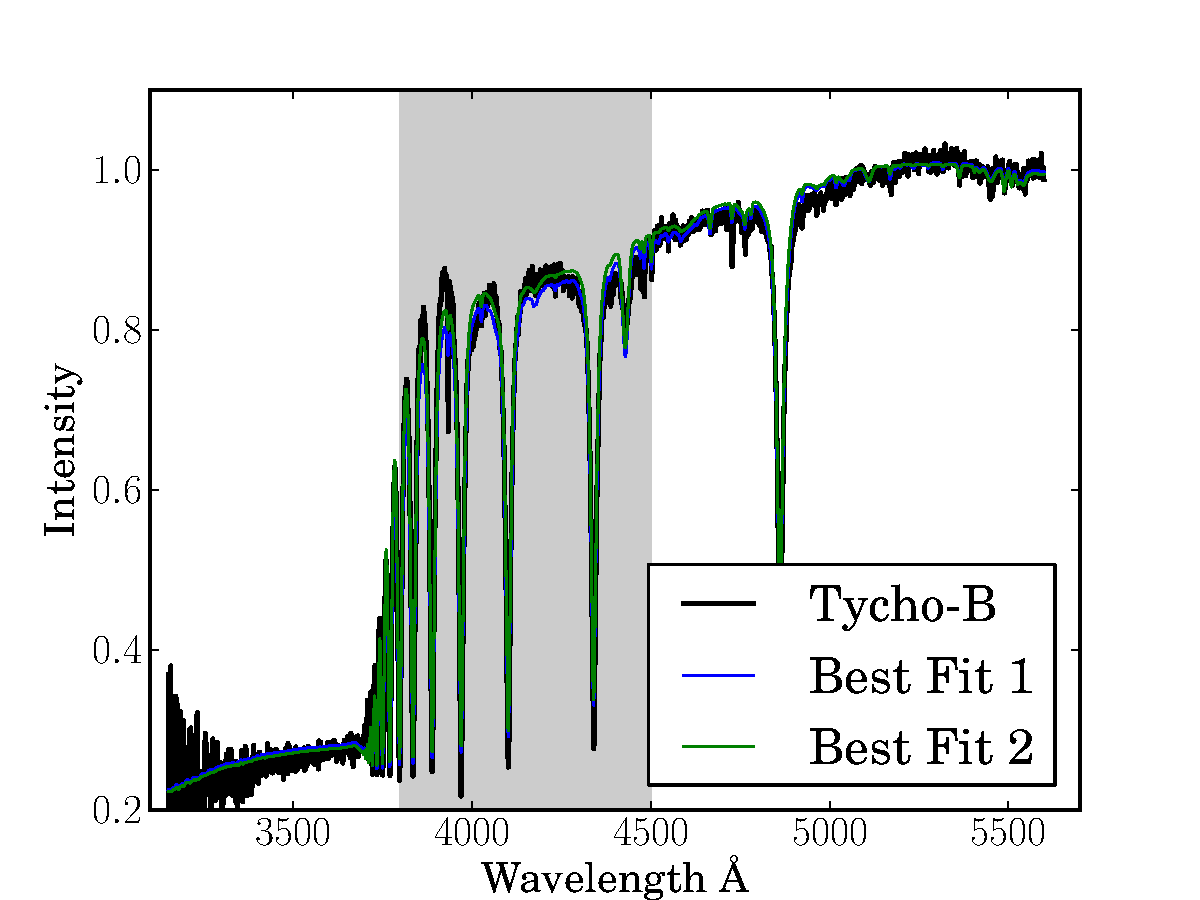
\includegraphics[width=1.\textwidth]{chapter_sn1572_hires/plots/starb_spec_comp.pdf} 

\caption[Fit of low resolution spectrum of Tycho-B]{The plot shows the normalized spectrum of \starb\ with the fit which excluded the spectral region between 3800--4500~\AA (Best Fit 1) and the fit with the problematic region (Best Fit 2). The region is marked with a grey shade.  }
\label{fig:starb_spec_comp}
\end{figure}

\subsection{Distances}
\label{sec:distance}
To measure the distance to the candidate stars we used colours and absolute magnitude from isochrones by  \citet{2004ApJ...612..168P}. We used the \gls{migrad} algorithm  \citep{James:1975dr} to find close matches of the measured values to \teff-\logg\ isochrones by varying the age of the isochrone.  Subsequently we calculate E(B-V) using the isochrone's colour and we extract a mass from the isochrone. The results can be seen in Table \ref{table:iso_dist}. To estimate the errors in all distance, reddening and mass we employed the \gls{mc}
method with 10,000 samples of \gls{teff} , \gls{logg}, \gls{feh}, B- and V-magnitude (see Figure  \ref{fig:mc_isochrone}).  Errors included in Table \ref{table:iso_dist} are the standard deviations of the Monte-Carlo sample. 
The data shows that all stars are compatible with the distance of the remnant. This is not unexpected as the uncertainties of the measurements in stellar parameters are relatively large.




\begin{figure}[htbp] %  figure placement: here, top, bottom, or page
   \includegraphics[width=0.5\textwidth]{chapter_sn1572_hires/plots/tycho-a-panel.pdf} 
   \includegraphics[width=0.5\textwidth]{chapter_sn1572_hires/plots/tycho-b-panel.pdf} 
   \includegraphics[width=0.5\textwidth]{chapter_sn1572_hires/plots/tycho-c-panel.pdf} 
   \includegraphics[width=0.5\textwidth]{chapter_sn1572_hires/plots/tycho-e-panel.pdf} 
   \includegraphics[width=0.5\textwidth]{chapter_sn1572_hires/plots/tycho-g-panel.pdf} 
   \caption[Distance, extinction and mass measurements in \sn{1572}{}]{The figures show error contours for distance, extinction and mass of the candidates. The lower right shows the optimal isochrone \citep{2004ApJ...612..168P}  for the measured values of \glsentryname{teff} and \glsentryname{logg}. }
   \label{fig:mc_isochrone}
\end{figure}


\ctable[
caption = {Distances, Ages and Masses of candidate stars},
label = {table:iso_dist}
]
{lcccccc}{}{\FL
Name&Mass& $\Delta$Mass & Age & $\Delta$Age & Distance& $\Delta$Distance\\
designation& M/M$_\odot$ & M/M$_\odot$ & Gyr & Gyr & kpc & kpc \ML 
%\startdata
\stara & 2.4 & 0.8 &0.7 & 2.3 & 1.4 & 0.8\\
\starb & 1.8 & 0.4 &0.8 & 0.3 & 1.8 & 0.8\\
\starc & 0.9 & 0.4 &10.0 & 3.4 & 5.5 & 3.5\\
\stare & 1.7 & 0.4 &1.4 & 1.1 & 11.2 & 7.5\\
\starg & 1.1 & 0.2 &5.7 & 2.1 & 3.7 & 1.5\LL
}

\section{Discussion}
\label{sec:sn1572_hires:discussion}

In our sample of six stars we find no star that can be unambiguously identified as a a donor star for SN1572. On the other hand none of the stars in the sample can be completely ruled out. 

\stara\ is a metal rich giant. It seems to be likely that \stara\ is a foreground star. Its principal redeeming feature as a donor star candidate is that it is located in the geometric center of the remnant, and that it has a relatively low gravity. \stara\ shows a very low spatial motion which is consistent with a giant donor star scenario. Its lack of rotation, however, is in conflict with said scenario. 
Taking all measurements into account we regard \stara\ to be a very weak candidate.

\starb's  high temperature, position at the center of the remnant, high rotational velocity and unusual chemical abundance made it a highly unusual candidate in the Tycho Remnant center. Despite the a posteriori unlikely discovery of such a star in the remnant center, Star B's high rotational velocity coupled with its low spatial velocity, seem to be in conflict with viable donor star scenario. 
These scenarios predict that the donor star will tidally couple to the white dwarf star before explosion, causing the rotation and spatial motion to be correlated post explosion (as discussed in \wek). The large rotation seen in \starb\ should accompanied by spatial motion, which is ruled out by the observations presented here, a problem we are unable to reconcile with \starb\ being the donor star. 

 \starc\ consists of two stars which are only resolved in HST images. It consists of a brighter bluer component and a dimmer redder component (difference of ~ one magnitude in all colors) (\rl). In our analysis we find a satisfying solution for the spectrum and suspect that this is from the bluer brighter component. 
For the brighter bluer component \starc\ is a metalpoor giant, probably located beyond the remnant. \starc\ similar to \stara\ might be compatible with a giant donor star scenario. It's lack of rotation and kinematics, however, make it an uninteresting candidate.

\stard\ is roughly ten times dimmer than the close star \starc\ ($\approx 0.6$\arcsec). Our tools to measure stellar abundances are not effective for spectra with a S/N less than 10. We however compared the stars by over plotting them and determined that \stard\ is similar to \starc. Similar to \starc\ we believe \stard\ to be a very weak candidate.

\stare\ is the most distant star in this set (11.2\,kpc). It seems to be similar to \starg\ in temperature, however is a subgiant. It is located 7\arcsec from the geometric center and has no unusual stellar parameters or kinematics. \citet{2007PASJ...59..811I} have looked at iron absorption lines in stellar spectra made by the remnant and found \stare\ to be unusual. They suggest that a star in the background would show blue and redshifted iron lines, a star inside the remnant would only show blueshifted iron lines.  A foreground star will not show any iron features from the remnant. \citet{2007PASJ...59..811I}  suggest that \stare\ only shows blue-shifted lines and thus is suggested as being in the remnant. We believe however that \stare\ is located far behind the remnant and suggest that a low column density on the receding side of the remnant could cause a lack of red-shifted iron features.  
In summary, a lack of rotation, kinematics and distance make it a very weak candidate.

\starg\ is located 30\arcsec\ from the X-Ray center which makes it the most remote object to the center in this work. This work confirms the radial velocity measured by \gh\ and \wek. Figure \ref{fig:dist_vr} shows the exepected distribution of radial velocities from the Bescan\c{c}on model of Galactic dynamics. \starg\ is not a significant outlier at the distance of the remnant as well as behind. 
In addition, this work has analysed the proper motion of stars around the center of SN1572. Figure \ref{fig:propmot_sn1572_hires} shows \starg\ to be a slight outlier, but also shows other stars to be outliers.
The kinematic features of a donor star might easily be lost in the kinematic noise of the Galaxy. \wek, however, suggested using post-explosion stellar rotation as a possible feature for a donor star. This work suggests that \starg\ has a rotation below the instrumental profile. 
We find \starg\ to be a sub-giant star with roughly solar temperature and metallicity.
\gh\ measure a slight Ni enhancement, which they believe to originate in the contamination from the ejecta. Figure \ref{fig:kobayashi06} compares our measurement of \starg\ to the distribution of Ni and finds it to be consistent with this distribution. In addition, we could not measure a significantly enhanced Lithium-abundance as suggested in \gh. 
Finally, we have measured the distance to \starg\ and believe it to be behind the remnant. Although our error bars make it consistent with the remnant.

In summary, we acknowledge that \starg\ has unusual kinematics. However, this kinematic predicts rotation for \starg\ which we do not observe (there are caveats however, see \wek). We have not  found a satisfying explanation for \starg's large distance to the geometric center. We suggest that \starg\, has the features consistent sub-giant background interloper.

\section{Conclusion}
\label{sec:sn1572_hires:conclusion}
This work did not detect an unambiguously identifiable donor star candidate. We acknowledge that \starb\ and \starg\ have unusual features, but there has been no conclusive explanation for all their parameters. Further theoretical predictions are needed to make a more precise distinction between donors and unrelated stars. 
 
Our observations provide a case that the Tycho SNR does not have a MS, SG, or RG donor star, but other possibilities remain. These include a Helium donor, such as the so-called Sub-Chandra explosions discussed by \cite{1995ApJ...452...62L, 2010ApJ...714L..52S}. These progenitor systems might leave behind a very faint and fast moving He star. Such a progenitor would probably evade detection, and would likely not leave behind traces, such as \gls{csi} with the remnant, or early light curve anomalies \citep{2010ApJ...708.1025K}. However, deep multi-epoch wide field optical images should catch any such star speeding away from the remnant center - these are observation not yet taken.
 Finally, a double degenerate progenitor, in most cases, does not leave behind a remnant , and is consistent with finding no donor star in Tycho SNR. 
 
\sn{1006}{}\ and \sn{1604}{}\ (Kepler's \gls{sn}) are two other \snia\ remnants in the Milky Way. \sn{1006}{}\ is far from the plane and shows no signs of \gls{csi}. \snr{1604}\ while far from the galaxy plane, shows \gls{csi} with its remnant, and has all the indications of what might be expected from a \gls{sds} of a \gls{mainsequence} or lower gravity star \citep{2011arXiv1103.5487C}. Observations of these remnant will better establish if there is a continued pattern to the unusual stars in \snia remnant centres, or whether the lack of viable donor stars persists in multiple systems.



